\section{Theoretical Analysis}
\label{sec:analysis}

In this section, a theoretical analysis of the previously shown circuit was conducted. 
An OP-AMP BandPass filter blocks the undesired frequencies, allowing only a certain bandwidth of frequencies to pass through. Besides that, it also amplifies the signal for these frequencies. As it is an active filter, transistors are used, apart from resistors and capacitors, with the purpose of amplifying the signal. In this laboratory, the 741 OP-AMP is used in an non inverting manner and the input signal is filtered.
\par
The transfer function for the circuit is:

\begin{equation}
	T(s) = \frac{R_1C_1s}{R_1C_1s + 1} \frac{R_3+R_4}{R_4} \frac{1}{R_2C_2s + 1},
	\label{eq:T}
\end{equation}

where the first part is the result of the high pass subcircuit, the second is due to the OP-AMP (assumig that $A_v = \infty$) and the third and last due to the low pass subcircuit after the OP-AMP.

The lower and upper cut-off frequencies, respectively, are given by the following expressions:

\begin{equation}
	\omega_L = \frac{1}{R_1C_1};
	\label{eq:WL}
\end{equation}
\begin{equation}
	\omega_H = \frac{1}{R_2C_2}.
	\label{eq:WH}
\end{equation}

Therefore, the central angular frequency, which corresponds to the geometric centre of there two frequencies above, is given by

\begin{equation}
	\omega_O = \sqrt{\omega_L \omega_H} = \sqrt{ \frac{1}{R_1C_1R_2C_2} };
	\label{eq:WO}
\end{equation}

The gain will be given when $s = j\omega_O$.

Finally, the input and output impedances, respectively, are given by:

\begin{equation}
	Z_I = Z_{R1} + Z_{C1} = R_1 + \frac{1}{j \omega_O C_1};
	\label{eq:ZI}
\end{equation}
\begin{equation}
	Z_O = Z_{R2} \parallel Z_{C2} = \frac{1}{\frac{1}{R_2} + j \omega_O C_2};
	\label{eq:ZO}
\end{equation}

The following table shows the theoretical results obtained using the previous formulas to optimise the merit: 

\begin{table}[h]
  \centering
  \begin{tabular}{|l|r|}
    \hline    
    {\bf Name} & {\bf Value} \\ \hline
    \input{../mat/MAT_IMP_tab}
  \end{tabular}
  \caption{The variables of type {\it impedance} and expressed in Ohm.}
  \label{tab:TEO_IMP}
\end{table}

We can observe that the output impedance of the circuit is non trivial, posing problems when considering connecting this amplifier to a low impedance load; this is the primary reason we have tested this circuit without a load connected ($R_L = \infty$).

\begin{table}[h]
  \centering
  \begin{tabular}{|l|r|}
    \hline    
    {\bf Name} & {\bf Value} \\ \hline
    \input{../mat/MAT_GAIN_tab}
  \end{tabular}
  \caption{Variables are adimentional.}
  \label{tab:TEO_RES}
\end{table}

The gain we see here is significantly lower than the requested 100. The problem arises with the limitations in the options of the resistors, since the gain comes from $\frac{R_3+R_4}{R_4}$, as seen in equation~\ref{eq:T}. With a low $R_4$, we could increase this gain significantly; unfortunatly, due to the necessary use of the $1k \Omega$ resistors in the filters, we are only left with $10k \Omega$ and $100k \Omega$ resistors, from each we take full advantage, pairing in series the $100k \Omega$ resistors (to create the biggest resistor possible) and in parallel the $10k \Omega$ resistor (to create the smallest possible resistor), which is not perfect. A simple solution to this problem would be to replace the $10k \Omega$ resistors with $2k \Omega$ ones. In that case, the pairing of $R_3=100k \Omega$ and $R_4=2k \parallel 2k \parallel 2k \Omega$ would be a almost perfect solution (given the limitations of discreet components).

The next figures show the frequency response obtained in this analysis. 

\begin{figure}[h] \centering
	\vspace{-0.3cm}
	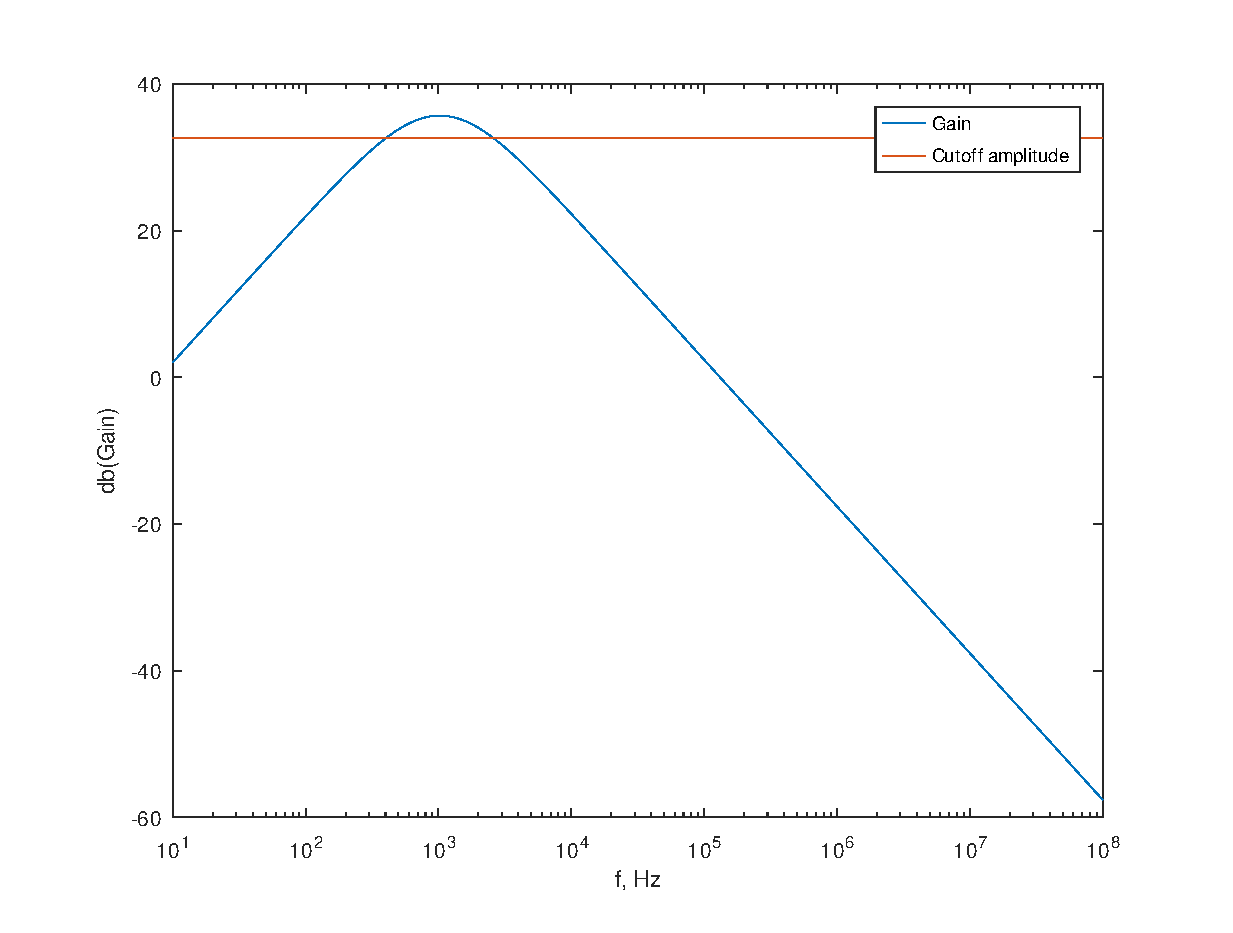
\includegraphics[height=8cm]{MAT_AB_AMP.eps}
	\caption{$db(v_{out})$ and $max(db(v_{out}))-3$.}
	\vspace{-0.1cm}
\end{figure}
\begin{figure}[h] \centering
	\vspace{-0.7cm}
	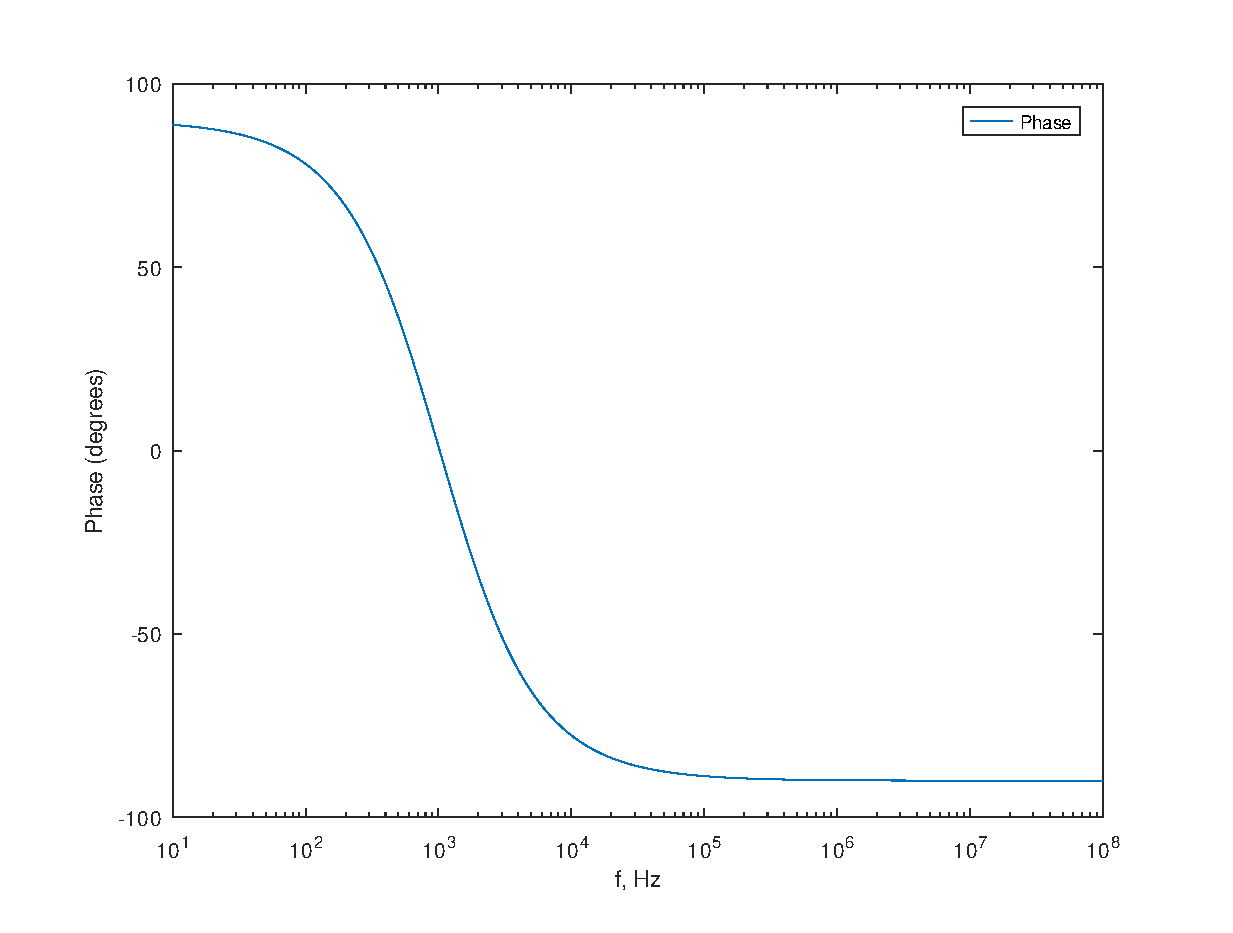
\includegraphics[height=8cm]{MAT_AB_PH.eps}
	\vspace{-0.1cm}
	\caption{Phasor of $v_{out}$, degrees.}
\end{figure}

We can see the two poles of the transfer function acting on the phase, subtracting 180 degrees from the initial phase and on the magnitude, only alowing a narrow set of frequencies to have a significant gain.